\begin{fullwidth}
\chapter[Assessing the impact of non-pharmaceutical interventions on SARS-CoV-2 transmission in Switzerland]{Assessing the impact of non-pharmaceutical\\ interventions on SARS-CoV-2 transmission\\ in Switzerland}
\label{ch:covid-switzerland-npi}
This chapter is based on a post-print version of:
\longfullcite{Lemaitre:AssessingImpactNonpharmaceutical:2020}, and J. Perez-Saez shares co-authorship of the work.
\section{Abstract}
Following the rapid dissemination of COVID-19 in Switzerland, large-scale non-pharmaceutical interventions (NPIs) were implemented by the cantons and the federal government between 28 February and 20 March 2020. Estimates of the impact of these interventions on SARSCoV-2 transmission are critical for decision making in this and future outbreaks. We here aim to assess the impact of these NPIs on disease transmission by estimating changes in the basic reproduction number ($R_0$) at national and cantonal levels in relation to the timing of these NPIs. We estimated the time-varying $R_0$ nationally and in eleven cantons by fitting a stochastic transmission model explicitly simulating within-hospital dynamics. We used individual-level data from more than 1000 hospitalised patients in Switzerland and public daily reports of hospitalisations and deaths. We estimated the national $R_0$ to be 2.8 (95\% confidence interval 2.1–3.8) at the beginning of the epidemic. Starting from around 7 March, we found a strong reduction in time-varying $R_0$ with a 86\% median decrease (95\% quantile range [QR] 79–90\%) to a value of 0.40 (95\% QR 0.3–0.58) in the period of 29 March to 5 April. At the cantonal level, $R_0$ decreased over the course of the epidemic between 53\% and 92\%. Reductions in time-varying $R_0$ were synchronous with changes in mobility patterns as estimated through smartphone activity, which started before the official implementation of NPIs. We inferred that most of the reduction of transmission is attributable to behavioural changes as opposed to natural immunity, the latter accounting for only about 4\% of the total reduction in effective transmission. As Switzerland considers relaxing some of the restrictions of social mixing, current estimates of time-varying $R_0$ well below one are promising. However, as of 24 April 2020, at least 96\% (95\% QR 95.7–96.4\%) of the Swiss population remains susceptible to SARS-CoV-2. These results warrant a cautious relaxation of social distance practices and close monitoring of changes in both the basic and effective reproduction numbers.
\end{fullwidth}

\section{Introduction}
As of 13 May 2020, the ongoing coronavirus disease 2019 (COVID-19) pandemic caused by severe acute respiratory syndrome coronavirus 2 (SARS-CoV-2) has resulted in more than 4.1 million cases and 280,000 deaths globally\cite{WHO:WHOSituationReport:2020}. Independent estimates of the basic reproduction number $R_0$ for SARS-CoV-2 from the initial phases of the epidemic in China, Europe and the US have generally ranged from 2–3 with doubling times on the order of 2–4 days. In response to the rapid increase in reported cases and hospitalisations, most countries have implemented nonpharmaceutical interventions (NPIs), including compulsory face mask use, border and school closures, quarantine of suspected and confirmed cases, up to population-wide home isolation\cite{HITCOVIDTeam:HealthInterventionsTracking:2020}. An observation study conducted in Hong Kong during this pandemic estimated that social distancing measures and school closures reduced COVID-19 transmission, as characterised by the effective reproductive number, by 44\%\cite{Cowling:ImpactAssessmentNonpharmaceutical:2020}. Comparable reductions have been observed in many different settings\cite{Flaxman:Report13Estimating:2020}. Making decisions around relaxing NPIs requires both a careful assessment of the level of pre-relaxation transmission (e.g., $R_0$) and quantification of the expected increase in transmission from relaxation of different NPIs. 

From the initial reported case on the 24 February to 29 April, Switzerland reported more than 24,400 laboratoryconfirmed COVID-19 cases and 1408 official deaths affecting all 26 cantons\cite{OFSP:RapportSituationEpidemiologique:2020}. The federal government issued a series of special decrees from 28 February banning gatherings of more than 1000 people culminating on March 20 recommended home isolation (fig. \ref{fig:covid-ch-data}). One month after the first NPI, daily confirmed case incidence had decreased from a peak of more than 1000 to a daily average of under 170 in the week of 20–26 April (fig. \ref{fig:covid-ch-data}). Initial reports have suggested a basic reproduction number ($R_0$) of 3.5 at the start of the epidemic, with a decrease of 85\% by March 20\cite[-3\baselineskip]{Flaxman:Report13Estimating:2020}.
\begin{figure*}\centering
  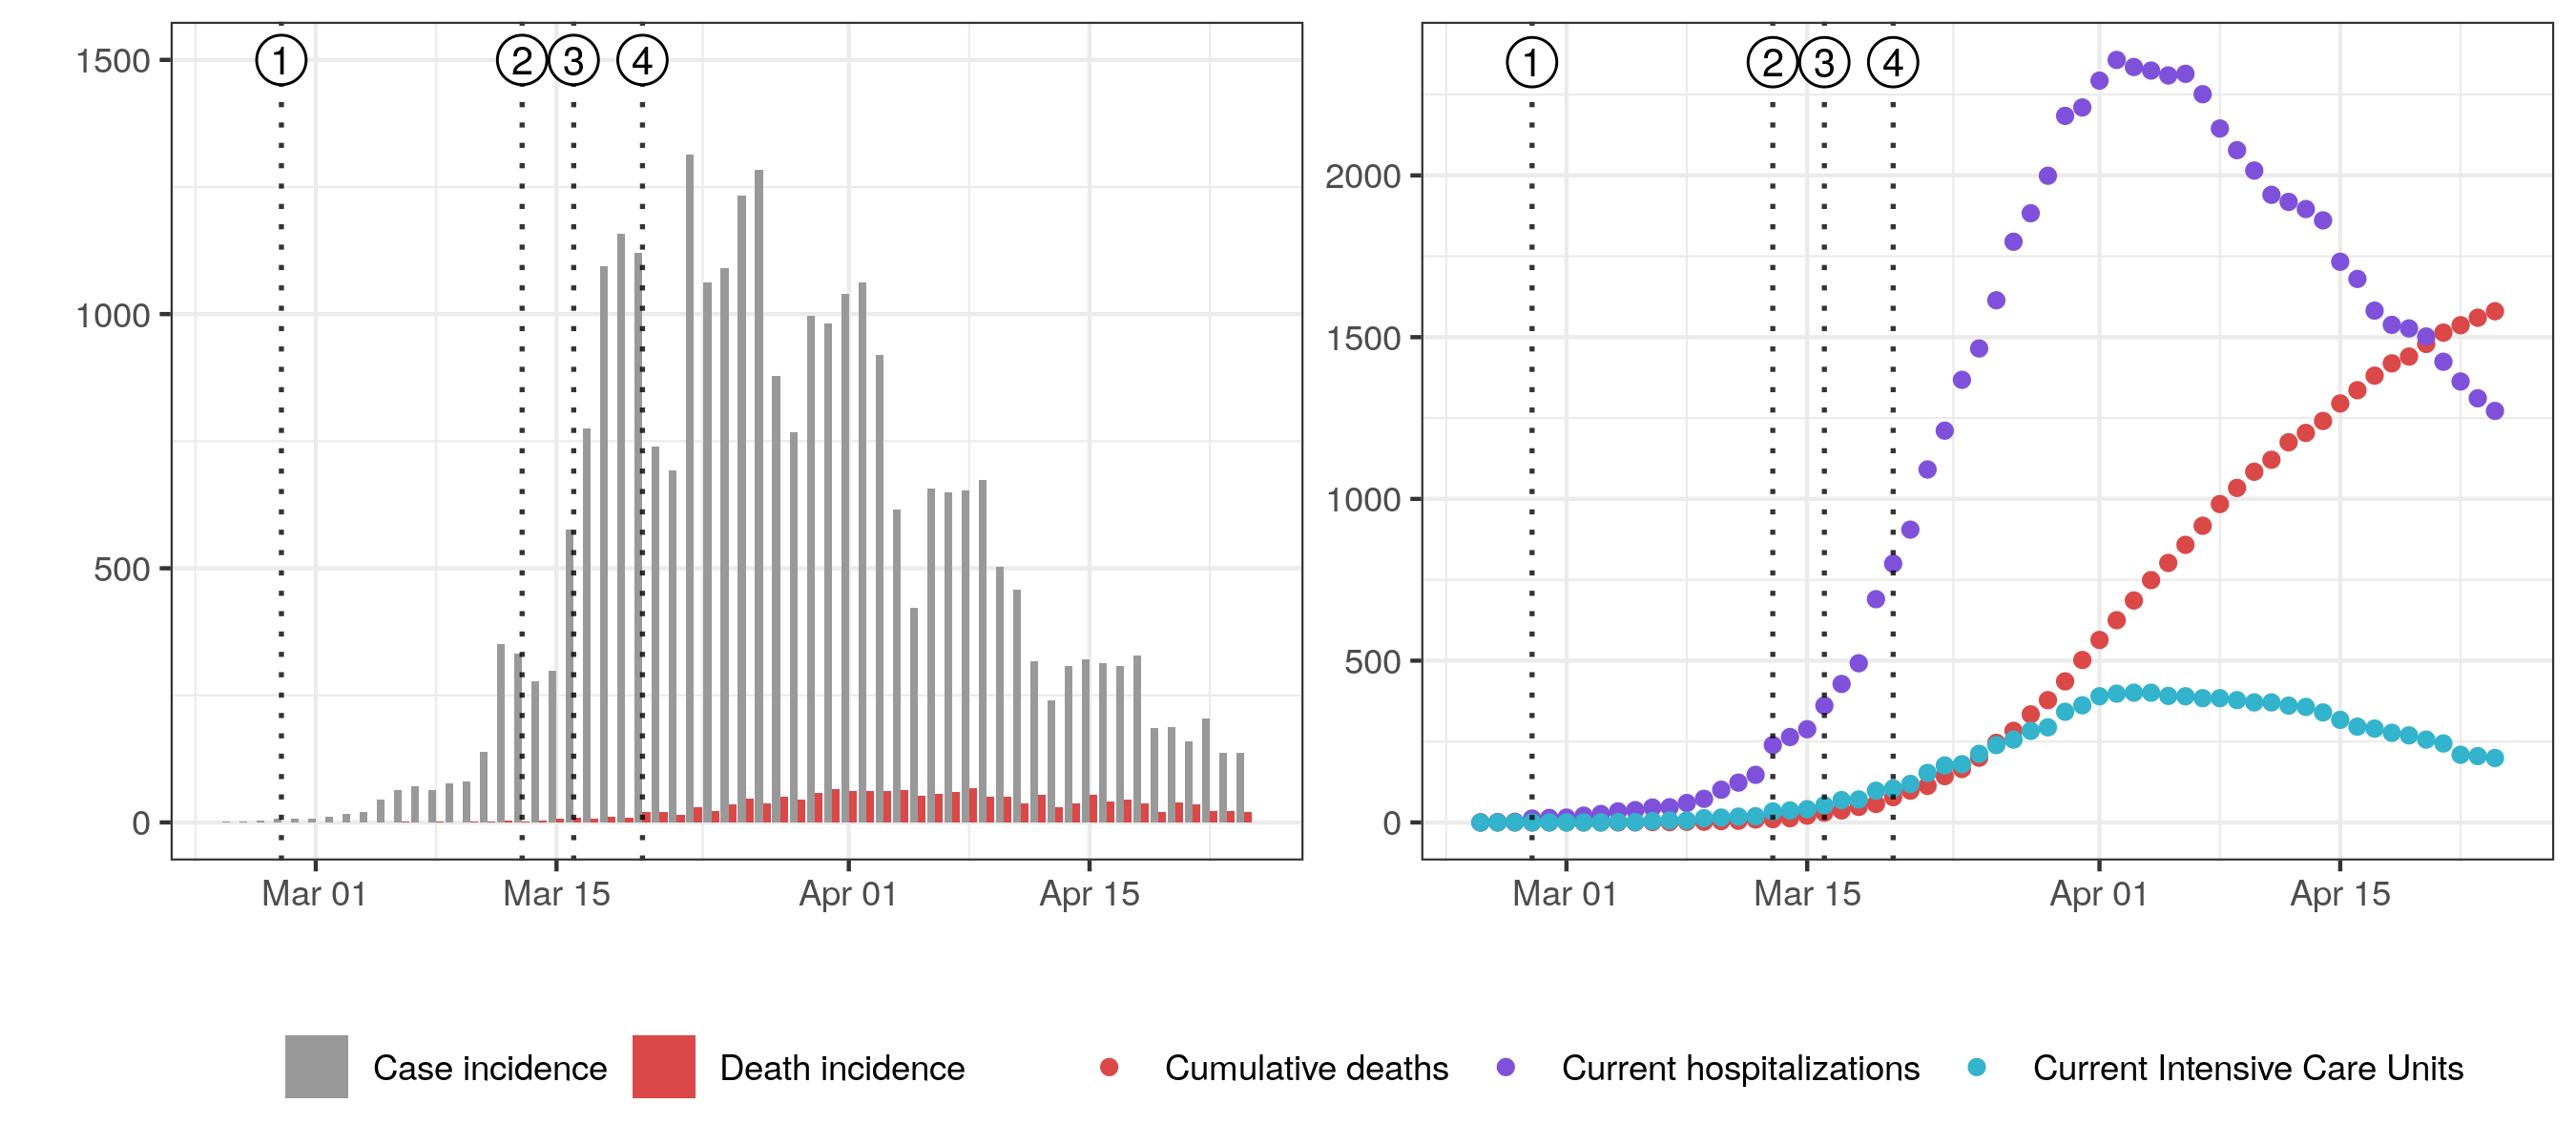
\includegraphics[width=\textwidth]{fig_covid-switzerland-npi/FIGURE_1.png}
  \caption[COVID-19 epidemic curve in Switzerland and timing of interventions.]{COVID-19 epidemic curve in Switzerland and timing of non-pharmaceutical interventions. Dotted lines indicate the issuing of NPIs: (1) ban on gatherings of more than 1000 people, (2) school closure, (3) closure of non-essential activities, and (4) ban on gatherings of more than five people. Left: Daily case incidence at time of reporting along with death incidence. Right: Current hospitalisations, intensive care units (ICUs) and cumulative deaths. Data from \textcite{Probst:DaenuprobstCovid19casesswitzerland:2020}, and may therefore present inconsistencies with official reports from the Federal Office of Public Health% due to reporting delays.
  }
  \label{fig:covid-ch-data}
\end{figure*}
 However, these estimates, part of a multicountry analysis of NPIs, relied on death incidence and did not account for specifics of the hospitalisation processes in Switzerland. 
Moreover, changes in $R_0$ were assumed to be on the date of NPI implementation, thus not allowing for the exploration of the relative timing between NPIs and changes in transmission. Furthermore, such delays might bias the estimate $R_0$. NPIs affecting daily activities such as school closures and gathering bans aim at having a direct impact on mobility patterns to reduce potentially infectious social contact. In other terms, the causal pathway from NPIs to transmission reduction is mediated by changes in mobility. Recent releases of mobility data from smartphone software providers give the possibility to study the associations between the implementation of movement-limiting measures, behavioural change and the related changes in $R_0$. Context-specific data on the degree and speed of compliance with these types of NPIs and associations with the observed decreases in $R_0$ could inform scenario-building should the future reinstatement of measures become necessary. Given that $R_0$ directly represents transmission potential, its quantification enables us to estimate the proportion of reduction in transmission attribuable to behavioral changes. In this sense, tracking of $R_0$ is more suited to study the impact of NPIs than the effective reproduction number (Reff), which is an aggregate measure of transmission capturing aspects of both infectious contacts and of population susceptibility. 

Here, we aimed at estimating changes in $R_0$ over the course of the epidemic at both the national and cantonal levels using detailed data on hospitalisations and deaths from Switzerland between 24 February and 24 April. To begin to understand the estimated changes in $R_0$, we explored its relationship with the timing of NPIs and human mobility estimates derived from cell phone data.

\section{Methods}
\subsection{Model and assumptions}
We developed a stochastic compartmental model of the COVID-19 epidemic and hospitalisation processes in each canton of Switzerland. We structure our model around the classical S, E, I and R compartments\cite{Kermack:ContributionMathematicalTheory:1927}. Namely, we consider that the population is divided in compartments depending on their status with regard to COVID-19. A susceptible individual (S) might be exposed after contact with infectious (I) individuals. Upon exposure, a formerly susceptible individual goes through an incubation period (E) before becoming infectious (I). The individual then recovers (R) and does not participate in transmission anymore. In addition to these dynamics, in the proposed framework some proportion of infectected invididuals develop severe disease and among those, some are hospitalised and may advance to needing the intensive care unit. Namely, infected individuals have some probability of developing severe symptoms which require hospitalization after a delay from symptom onset ($I_h$). Hospitalization can lead to recovery or death, either through normal hospitalization ($H_{s}$ and $H_d$ respectively) or passing through Intensive Care Units (ICUs, compartments $U_{s}$ and $U_d$ respectively). Data from the canton of Vaud show a high proportion of deaths outside of hospitals ($\approx 50\%$), we therefore also include a pathway from infection to death without passing through hospitalization, with compartment $I_d$ for severly infected that do not seek care. 
 (U compartments). Hospitalisation can progress to discharge, ICU or death and those in the ICU (U compartments) can either be discharged or die (model diagram in fig. \ref{fig:covid-ch-diagram}).  The model is implemented as a hidden markov model using the pomp R package\cite[-8\baselineskip]{King:StatisticalInferencePartially:2015}. 
 \begin{figure}[!htb]
\begin{center}
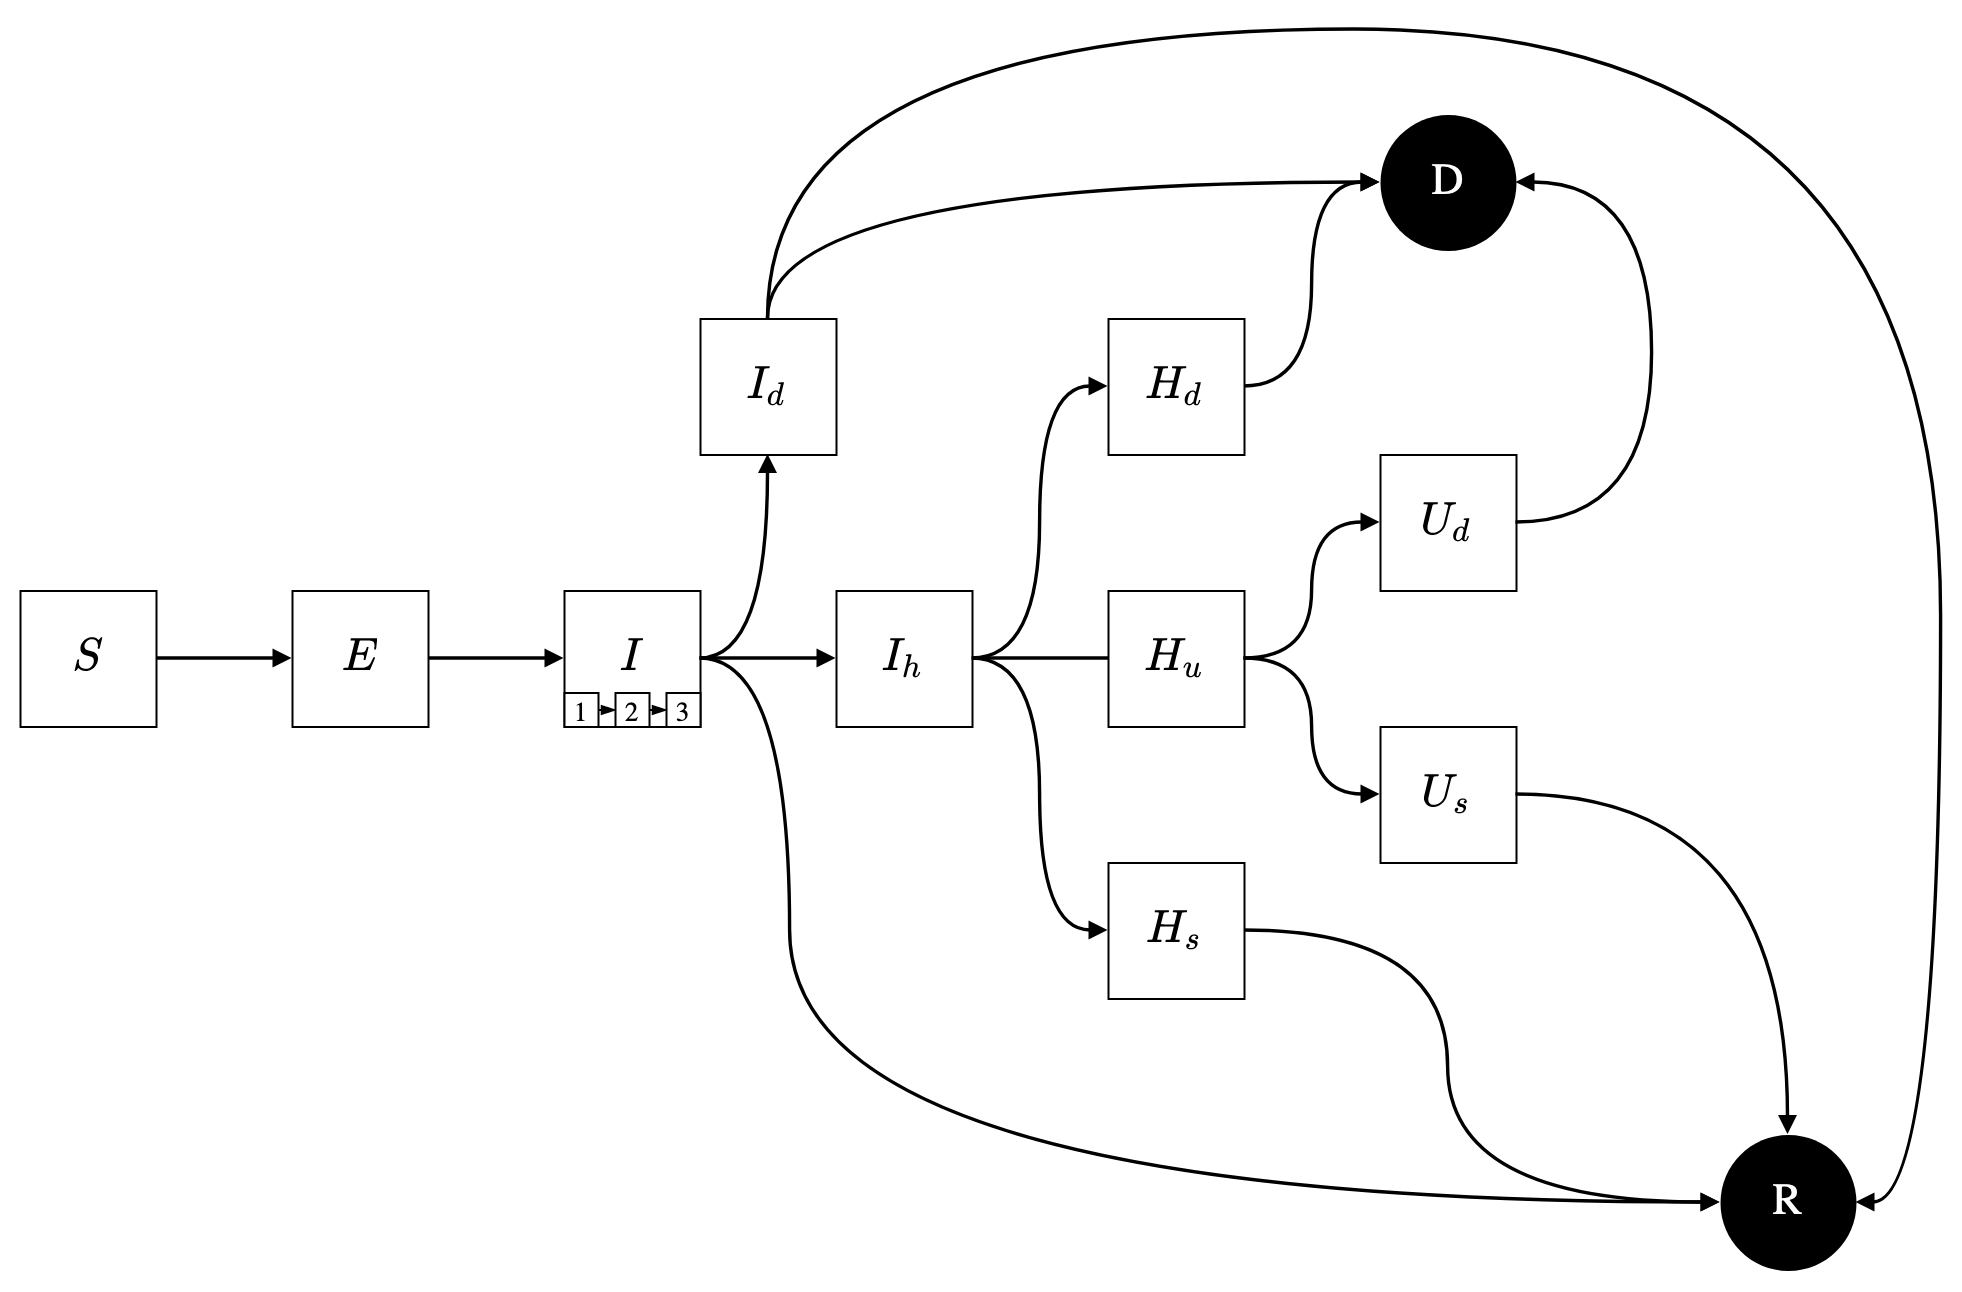
\includegraphics{fig_covid-switzerland-npi/fig_supp/diagram.png}
\caption[Schematic diagram of COVID-19 transmission and hospitalization processes.]{Schematic diagram of COVID-19 transmission and hospitalization processes. There are two sinks: Death $D$ and recovered $R$. Each stage with regard to the disease may be implemented with several compartments (subscript numbered boxes) to better represent the time distribution spent in that stage. The time spent in the observable hospitalization states were used to define the number of stages in each compartment by fitting Erlang distributions to the data of canton de Vaud. To account for right-censoring we do not fit directly to observed times to events but rather to the estimated log-normal distributions described in the survival analysis section above. We fit the rate parameter of the Erlang distributions for shape parameters between 1 and 10 by minimizing the Kullback-Leibler (KL) divergence between the Erlang and estimated log-normal distributions. The final fit was taken to be the one with the smallest KL-divergence.}
\label{fig:covid-ch-diagram}
\end{center}
\end{figure}
We used only hospitalisation and death data (see below), and so we do not need to explicitly model a latent stage where individuals are still asymptomatic but infectious\cite[-8\baselineskip]{Ganyani:EstimatingGenerationInterval:2020,He:TemporalDynamicsViral:2020, Liu:ContributionPresymptomaticInfection:2020}. Instead, we parameterise the model assuming a mean generation time of 5.2 days\cite[-2\baselineskip]{Ganyani:EstimatingGenerationInterval:2020}, and an exposed and non-infectious duration of 2.9 days\cite[-1\baselineskip]{He:TemporalDynamicsViral:2020}, yielding a mean duration of 4.6 days in the infectious compartments. The exhaustive description of model transitions and parameters are presented in the postprint supplementary table 3 of appendix 1. We assumed that 7.5\% of infections were severe and would require hospitalisation, that 50\% of deaths happened outside of hospitals (data from Vaud described in \textsc{Chapter 6}, and data from Geneva collected from OpenZH), that 16\% of those hospitalised would die (data from Vaud, supplementary fig. \ref{fig:covid-ch-r0}), and that the infection fatality ratio (IFR) was 0.75\%, which is in the range of published estimates\cite[-4\baselineskip]{Verity:EstimatesSeverityCoronavirus:2020, Russell:EstimatingInfectionCase:2020}. We used individual-level data on hospitalised cases from the canton of Vaud to estimate the distribution of time spent in the hospital and in the intensive care unit (ICU). We estimated times to discharge and death using survival models that account for right-censoring of observations (see \textsc{Chapter 6}). The number of compartments for each hospitalisation state was based on distribution of timings from the Vaud data. 
\subsection{Data and Inference} 
\paragraph{Dataset} We use curated data from OpenZH\cite[3\baselineskip]{openZH:OpenZHCovid19:2020} up to 24 April. This dataset included, by canton, the number of currently hospitalised COVID patients, and the cumulative numbers of deaths, cases and hospital discharges. The latter were not available for all cantons. For our cantonal estimate, we focused on cantons that had enough cases and data to obtain meaningful results, keeping 11 of the 26 cantons (Bern, Basel-Landschaft, Basel-Stadt, Fribourg, Geneva, Jura, Neuchâtel, Ticino, Vaud, Valais and Zurich). These cantons account for 66\% of the Swiss population. Our national estimate used curated national aggregate data and thus encompassed all cantons\cite{Probst:DaenuprobstCovid19casesswitzerland:2020}. We fitted unknown parameters of our models using maximum likelihood inference through iterated filtering\cite{Ionides:InferenceDynamicLatent:2015}. We did not attempt to include confirmed case data into the observation model because of the heterogeneous testing strategies adopted across cantons and over time. We therefore fitted the model to death incidence and changes in current hospitalisations using appropriate likelihood functions:
\begin{equation}
\begin{split}
 \text{deaths}(t) &\sim \text{Poisson}(\Delta D(t)) \\
\Delta  \text{hosp}(t) &\sim \text{Skellam}(\Delta H(t), \Delta D_H(t) + \Delta R_H(t)) \\
\end{split}
\end{equation}
\noindent where, $\Delta D(t)$, $\Delta H(t)$, $\Delta D_H(t)$, $\Delta R_H(t)$ are respectively the number of new deaths, hospitalized, and deaths and discharged from hospitals at time $t$, and $\Delta hosp(t)$ is the difference between the number of current hospitalizations at times $t$ and $t-1$, for which we choose a Skellam distribution\footnote{which represents the difference between two independent random variables, each Poisson-distributed. See \fullcite{Skellam:FrequencyDistributionDifference:1946}.}. The full log-likelihood of the observation model was taken as the sum of the individual log-likelihoods of the $\Delta hosp(t)$ and of the $deaths(t)$. 
We calibrate the model separately for each canton on the daily death and hospitalization until April 24. Hospitalisation incidence data at the cantonal level would have provided more information, but we were unable to access these data. Fitting to hospitalisation incidence data, which we had access to in the canton of Vaud, yielded similar results to those when changes in current hospitalisations were used. The majority of model parameters was either derived from Vaud data or from the litterature (see postprint supplementary), it enables the identifiability of the reproduction number $R_0$.s 
 
 \paragraph{Reproduction number estimation} Time-varying basic reproduction numbers $R_0$ were estimated following a similar approach to Cazelles et al.\cite{Cazelles:AccountingNonstationarityEpidemiology:2018}, recently applied to COVID-19 transmission in Hubei\cite{Kucharski:EarlyDynamicsTransmission:2020}. The method aims at inferring the time series of $R_0$\footnote{As mentionned, we compute $R_0$, not $R_{eff}$ as our method estimates the basic reproduction number, \ie the expected number of infections generate by one infected individual in a fully susceptible population. To do so, we explicity model the susceptible and recovered population while other methods usually compute the effective reproduction number in the population.} that yields model dynamics that are in best agreement with the whole set of available observations. As such, the value of $R_0$ at a given point in time is informed by the whole data, and therefore does not have the limitations of being either “forward looking” or “backwards looking” as it is the case of commonly used statistical methods applied for this purpose\cite{Wallinga:DifferentEpidemicCurves:2004,Cori:NewFrameworkSoftware:2013}. 

 We model time-varying $R_0(t) = \beta(t)/(3r_I)$ as a geometric random walk defined by its calibrated variance, where $\beta$ is the transmission parameter and $1/(3r_I)$ is the mean duration spent in the infectious compartments $I_1$ to $I_3$. The force of infection is expressed in terms of $\beta(t)$ in the model. Given the state of the system at time \(t\), \(\mathcal{X}_t\), the transition $S \longrightarrow E$ model reads:

\begin{gather}
\label{eq:stochsys}
\begin{aligned}
    \mathbb{P}\left[ \Delta N_{SE}(t) = 1 \right|\mathcal{X}_t] &=  \beta(t)  \frac{I_1(t) + I_2(t) + I_3(t)}{P} S(t) \Delta t + o(\Delta t)\\
    \end{aligned}
\end{gather}


Once the time series was inferred, we assessed the timing and slope of changes in $R_0$ by using linear changepoint models\cite{Lindelov:McpPackageRegression:2020}. The null model corresponded to a linear decrease between two plateaus corresponding to the baseline value at the start of the epidemic and a low value after the implementation of NPIs. To allow for different slopes in the decreasing phase of $R_0$, we also fitted models with one and two additional breakpoints (corresponding to two and three different slopes), and the best model was selected using Bayesian model selection based on leave-one-out crossvalidation (details in section 6 of appendix 1). We contrasted the estimated changes in $R_0$ with changes in activity-related mobility data produced by Google\cite{GoogleLLC:GoogleCOVID19Community:2020}. Changes in activity were expressed as relative changes with respect to a baseline computed as the median over a 5-week period from 3 January to 6 February. Mobility changes were computed for different categories: grocery and pharmacy, parks, transit stations, retail and recreation, residential, and workplace. Mobility estimates were based on smartphone-based geo-location location data (GPS, WiFi connections, Bluetooth) from users who activated Location History for their Google Account. These data were used to determine changes in the number of visits to and length of stays in locations categorised into the above-mentioned types. The dataset therefore only covers a sample of the Swiss population who use smartphones, the latter representing around 80\% of the total population in 2020\cite{ODea:SmartphoneUsersSwitzerland:2020}. We used linear interpolation to fill gaps in the dataset, and we applied a 7-day moving average to smooth out weekly seasonality in activities. We computed the cross-correlation between changes in $R_0$ and the averaged changes in each type of activity up to a lag of 10-days. Changes in $R_0$ were computed based on location-specific baselines taken as the mean value of $R_0$ from the beginning of the simulations, 5 days before the first reported case in each canton, until 8 March. As for $R_0$ we employ changepoint models to identify dates of change in mobility patterns. \marginnote[-5\baselineskip]{All data and code except for individual hospitalisation data from Canton of Vaud have been deposited on Zenodo (\url{doi.org/10.5281/zenodo.3862075}). The change point analysis, model fit and additional results are omitted from this thesis and may be found in the supplementary informations of \parencite{Lemaitre:AssessingImpactNonpharmaceutical:2020}}


\section{Results}
\begin{figure*}\centering
  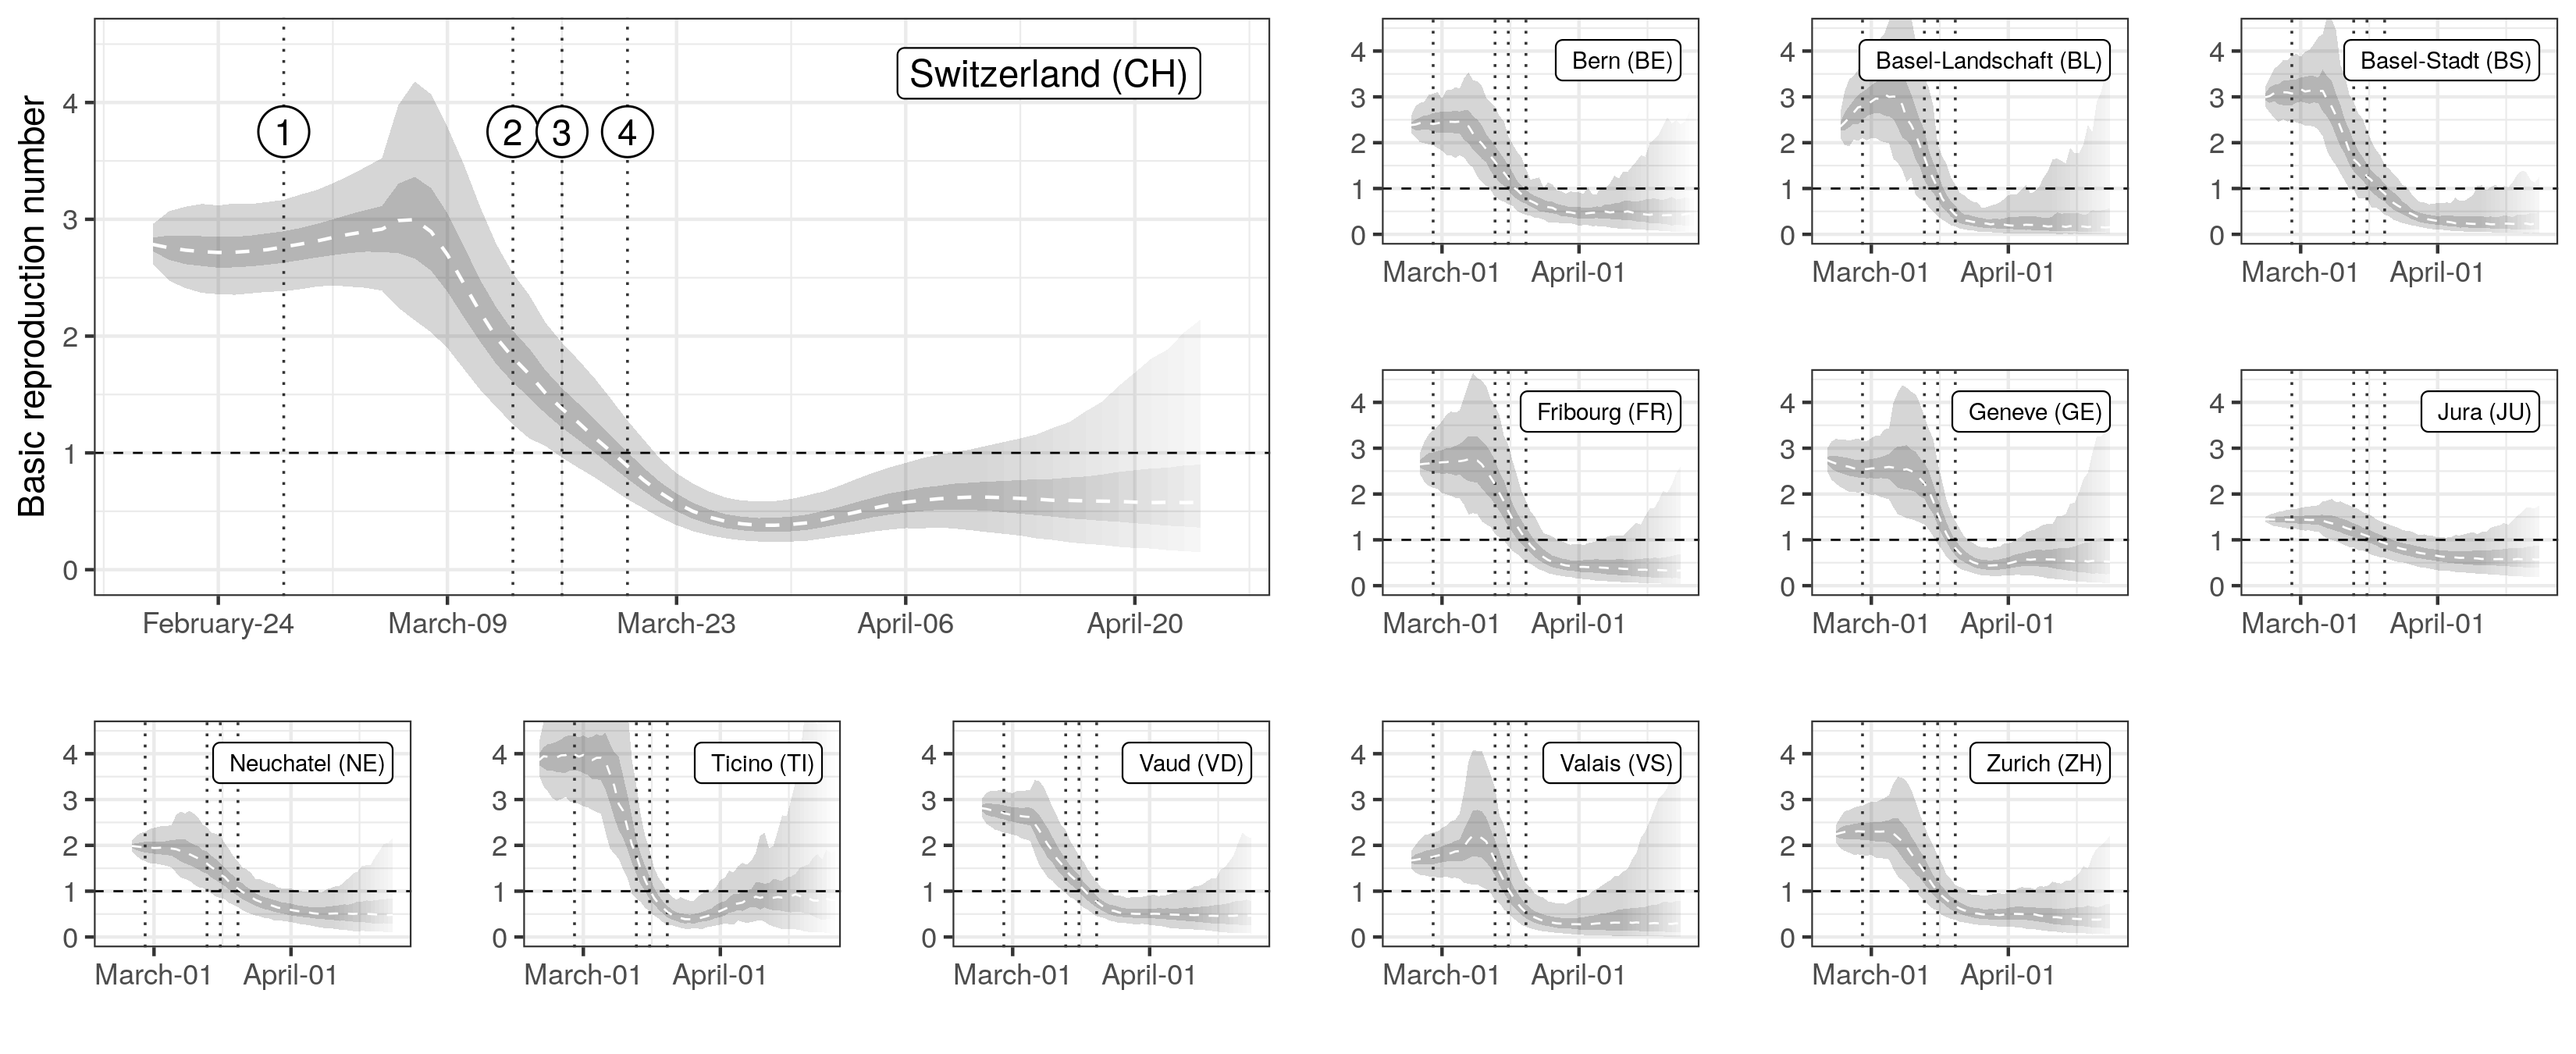
\includegraphics[width=\textwidth]{fig_covid-switzerland-npi/FIGURE_2.png}
  \caption[Estimates of changes in the basic reproduction number $R_0$.]{Estimates of changes in the basic reproduction number $R_0$. Median (dashed line), IQR (dark gray) and the 95\% QR (light gray) of the estimated time series of $R_0$ are shown for each canton. Vertical dotted lines indicate the issuing of NPIs as described in figure 1. Transparency at the end of the time series indicates increasing uncertainty (style inspired by CMMID).}
  \label{fig:covid-ch-r0}
\end{figure*}
Overall, we found that over the study period $R_0$ trends followed a common trajectory nationally and across cantons, starting with a high plateau ($R_0$ >2) in the early stage of the epidemic followed by a rapid reduction starting at the beginning of March, and reaching a low and stable value ($R_0$ <1) from end of March onwards (fig. \ref{fig:covid-ch-r0}). We estimated that at the beginning of the epidemic $R_0$ was 2.8 (95\% confidence interval [CI] 2.06–3.83) at the national level, with cantonal-level values ranging from 2.5 to 3.1 (postprint supplementary table 5, appendix 1). The onset of the reduction was estimated to be between 4 March (Basel-Stadt and Vaud) and 11 March (Geneva and Valais) at the cantonal level and on 7 March at the national level (postprint supplementary fig. 11). Overall we found strong support for the reduction in $R_0$ starting before school closures on 13 March (probability 0.99 at the national level, supplementary fig. 11). Once started, we estimated a strong decrease in $R_0$ at the national (reduction of 0.16/day) and cantonal levels (between 0.14/day in Jura to 0.18/day in Basel-Landschaft) (fig. \ref{fig:covid-ch-r0}). We did not find strong support for changes of slope during the decrease phase at either at the national or cantonal levels except for Bern, Basel-Stadt and Vaud, for which additional changes in slopes were inferred towards the stabilisation of $R_0$ at low values (postprint supplementary table 7).\marginnote[0\baselineskip]{Additional results may be found in the supplementary informations of \parencite{Lemaitre:AssessingImpactNonpharmaceutical:2020}} We estimated that $R_0$ in Switzerland dropped below 1 on 19 March (95\% CI 16–22 March) with individual cantons meeting this threshold between 16 March (Basel-Stadt) and 20 March (Neuchâtel) (postprint supplementary fig. 10). We estimated the probability that $R_0$ had already fallen below one was low when schools closed on 13 March (national 0.006, cantonal from 0 in Geneva to 0.23 in Basel-Landschaft), and high by the time gatherings of five people or more were banned on 20 March (national 0.92, cantonsal from 0.52 in Neuchâtel to 0.99 in Ticino) (postprint supplementary fig. 9). The estimated plateau value of $R_0$ after the reduction, that is, from 29 March to 10 April, was of 0.4 (95\% quantile range [QR] 0.3–0.6) at the national level, with median values at the cantonal level ranging from 0.2–0.7 (postprint supplementary table 5). At the national level, $R_0$ was reduced by 86\% (95\% QR 79–90\%), with median reductions ranging from 53\% (Jura) to 92\% (Basel-Stadt) at the cantonal level. A gradual reduction in $R_0$ leading to values below one around the third week of March is consistent with the observed reduction of confirmed case incidence in early April, when we take into consideration the delays due to the incubation period, with median of 5.2 days\cite[-5\baselineskip]{Lauer:IncubationPeriodCoronavirus:2020}, and between symptom onset and reporting\cite[-2\baselineskip]{Bi:EpidemiologyTransmissionCOVID19:2020}. Similarly, the inflection in the number of current hospitalisations and ICU usage in early April also supports $R_0$ dropping below one in mid-March. 
\begin{figure*}\centering
  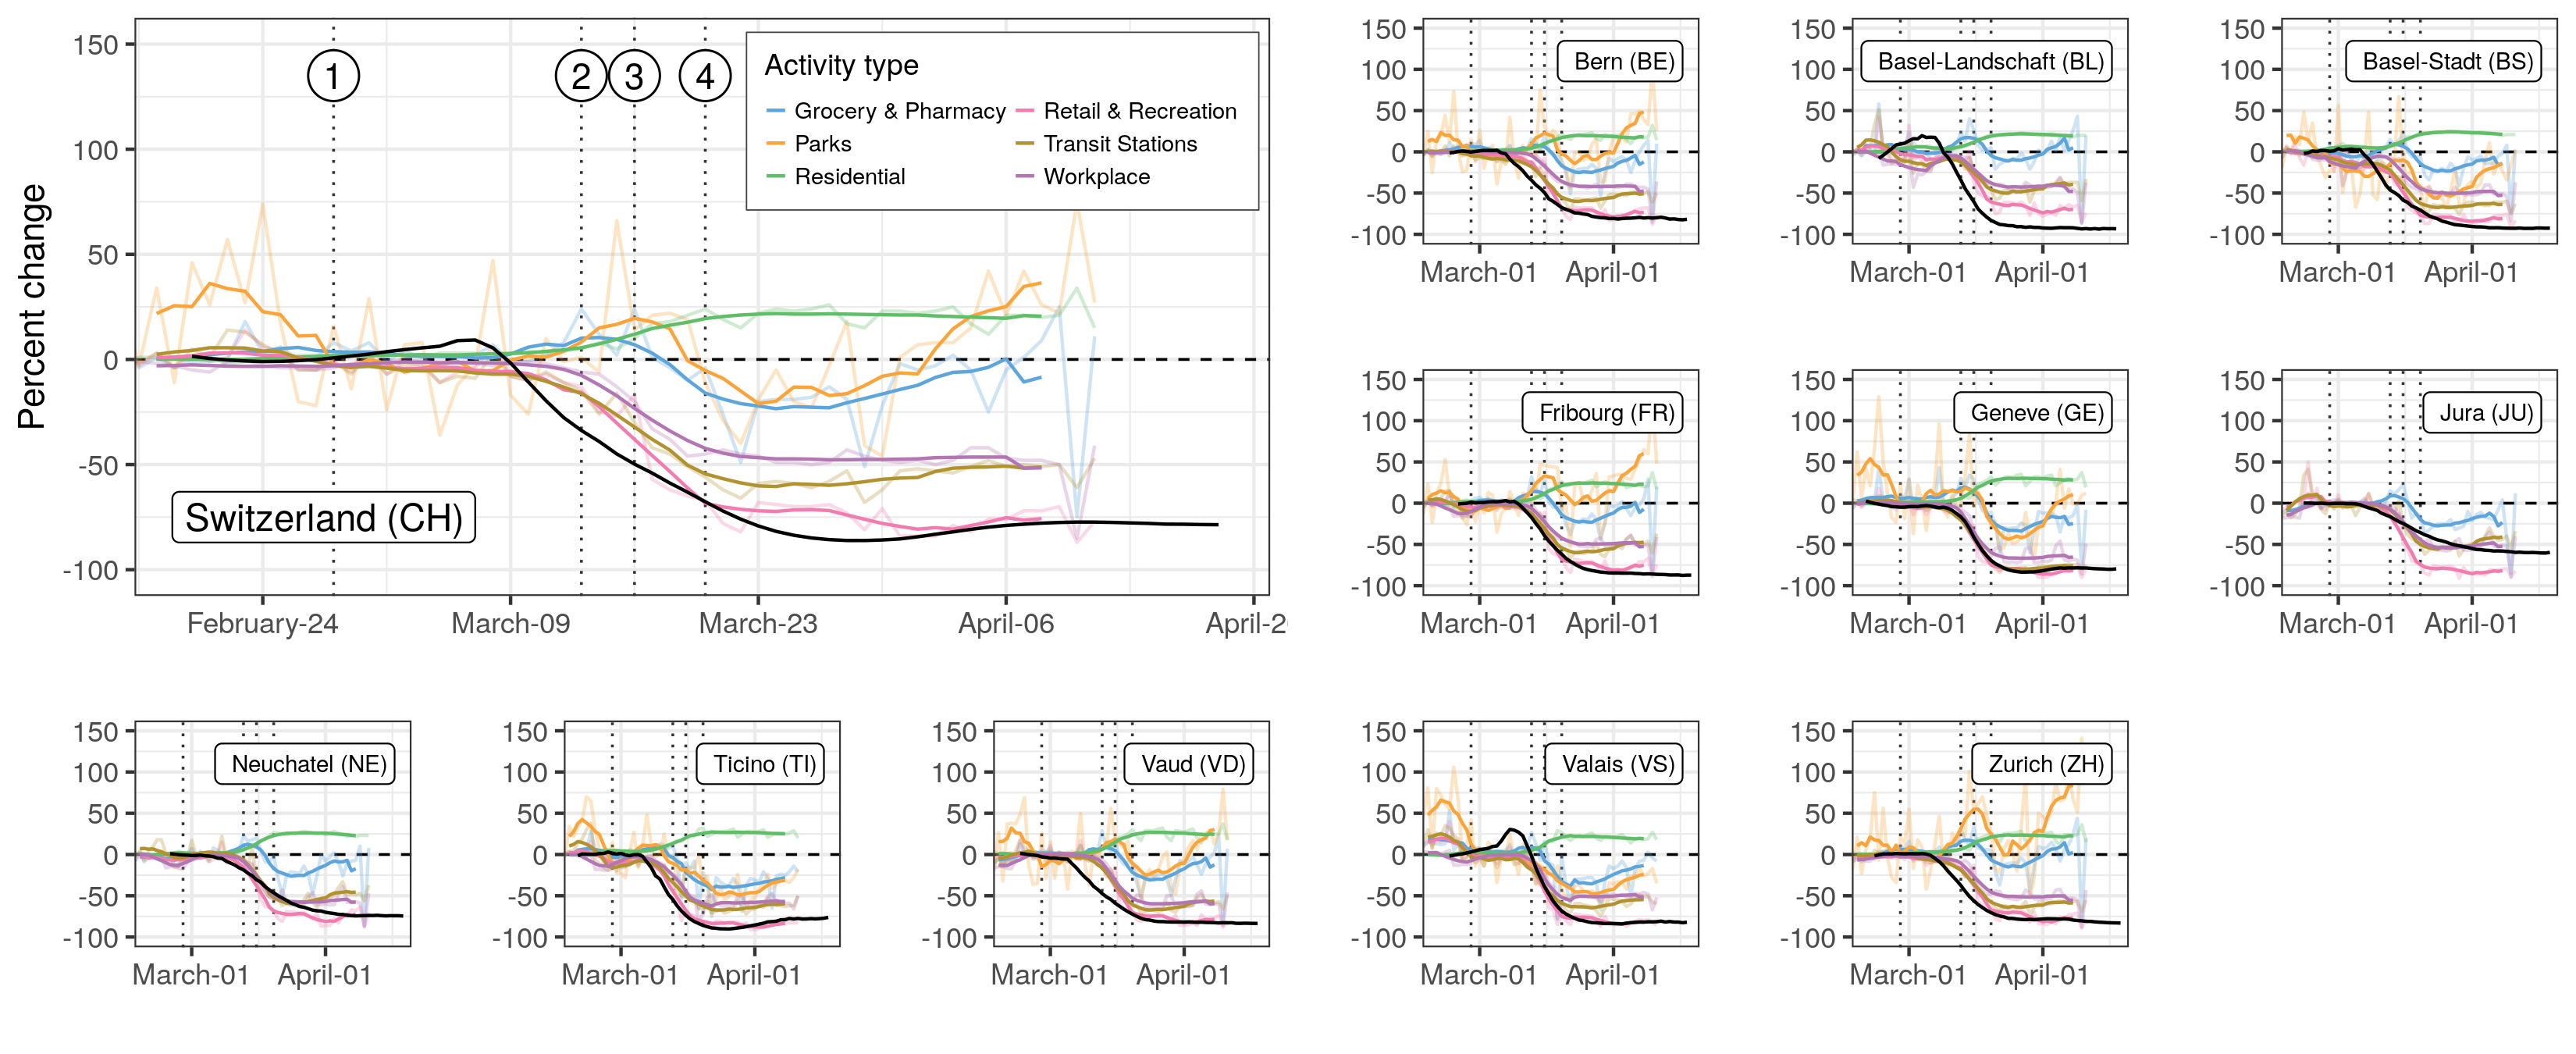
\includegraphics{fig_covid-switzerland-npi/FIGURE_3.png}
  \caption[Changes in mobility patterns and R0.]{Changes in mobility patterns and R0.Changes in mobility with respect to baseline are shown by activity type in terms of the daily values (transparent lines) and 7-day rolling mean (full lines), against the median estimate of R0 (black line). Vertical dotted lines indicate the issuing of NPIs: (1) ban on gatherings of more than 1000 people, (2) school closure, (3) closure of non-essential activities, and (4) ban on gatherings of more than five people.}
  \label{fig:covid-ch-mobility}
\end{figure*}

Activity-related mobility patterns changed markedly in all cantons since the beginning of the epidemic (fig. \ref{fig:covid-ch-mobility}). Mobility related to work, retail and recreation, and transit stations dropped by 50\% to 75\% at the national level, with cantonal-level reductions ranging from 30\% to 80\% depending on activities. Residential-related mobility increased across cantons between 20\% and 30\%. We found strong support for mobility changes starting simultaneously for all activity types within each canton. We estimated that changes in mobility started between 6 and 14 March for all cantons (postprint supplementary fig. 12), thus finding strong support for changes starting before school closure on 13 March (national-level mean probability across activities 0.70, cantonal range 0.55–0.99). Based on our changepoint models, we find that reductions in $R_0$ likely started (probability 0.76) before observed reductions in mobility at the national level and across cantons (fig. \ref{fig:covid-ch-mobility}). Changes in $R_0$ were highly correlated with changes in mobility, the strongest associations being with mobility related to work, transit stations, retail and recreation, and residential (cross-correlations >0.9 in all cantons and nationally, fig. \ref{fig:covid-ch-timing}). 
\begin{figure*}\centering
  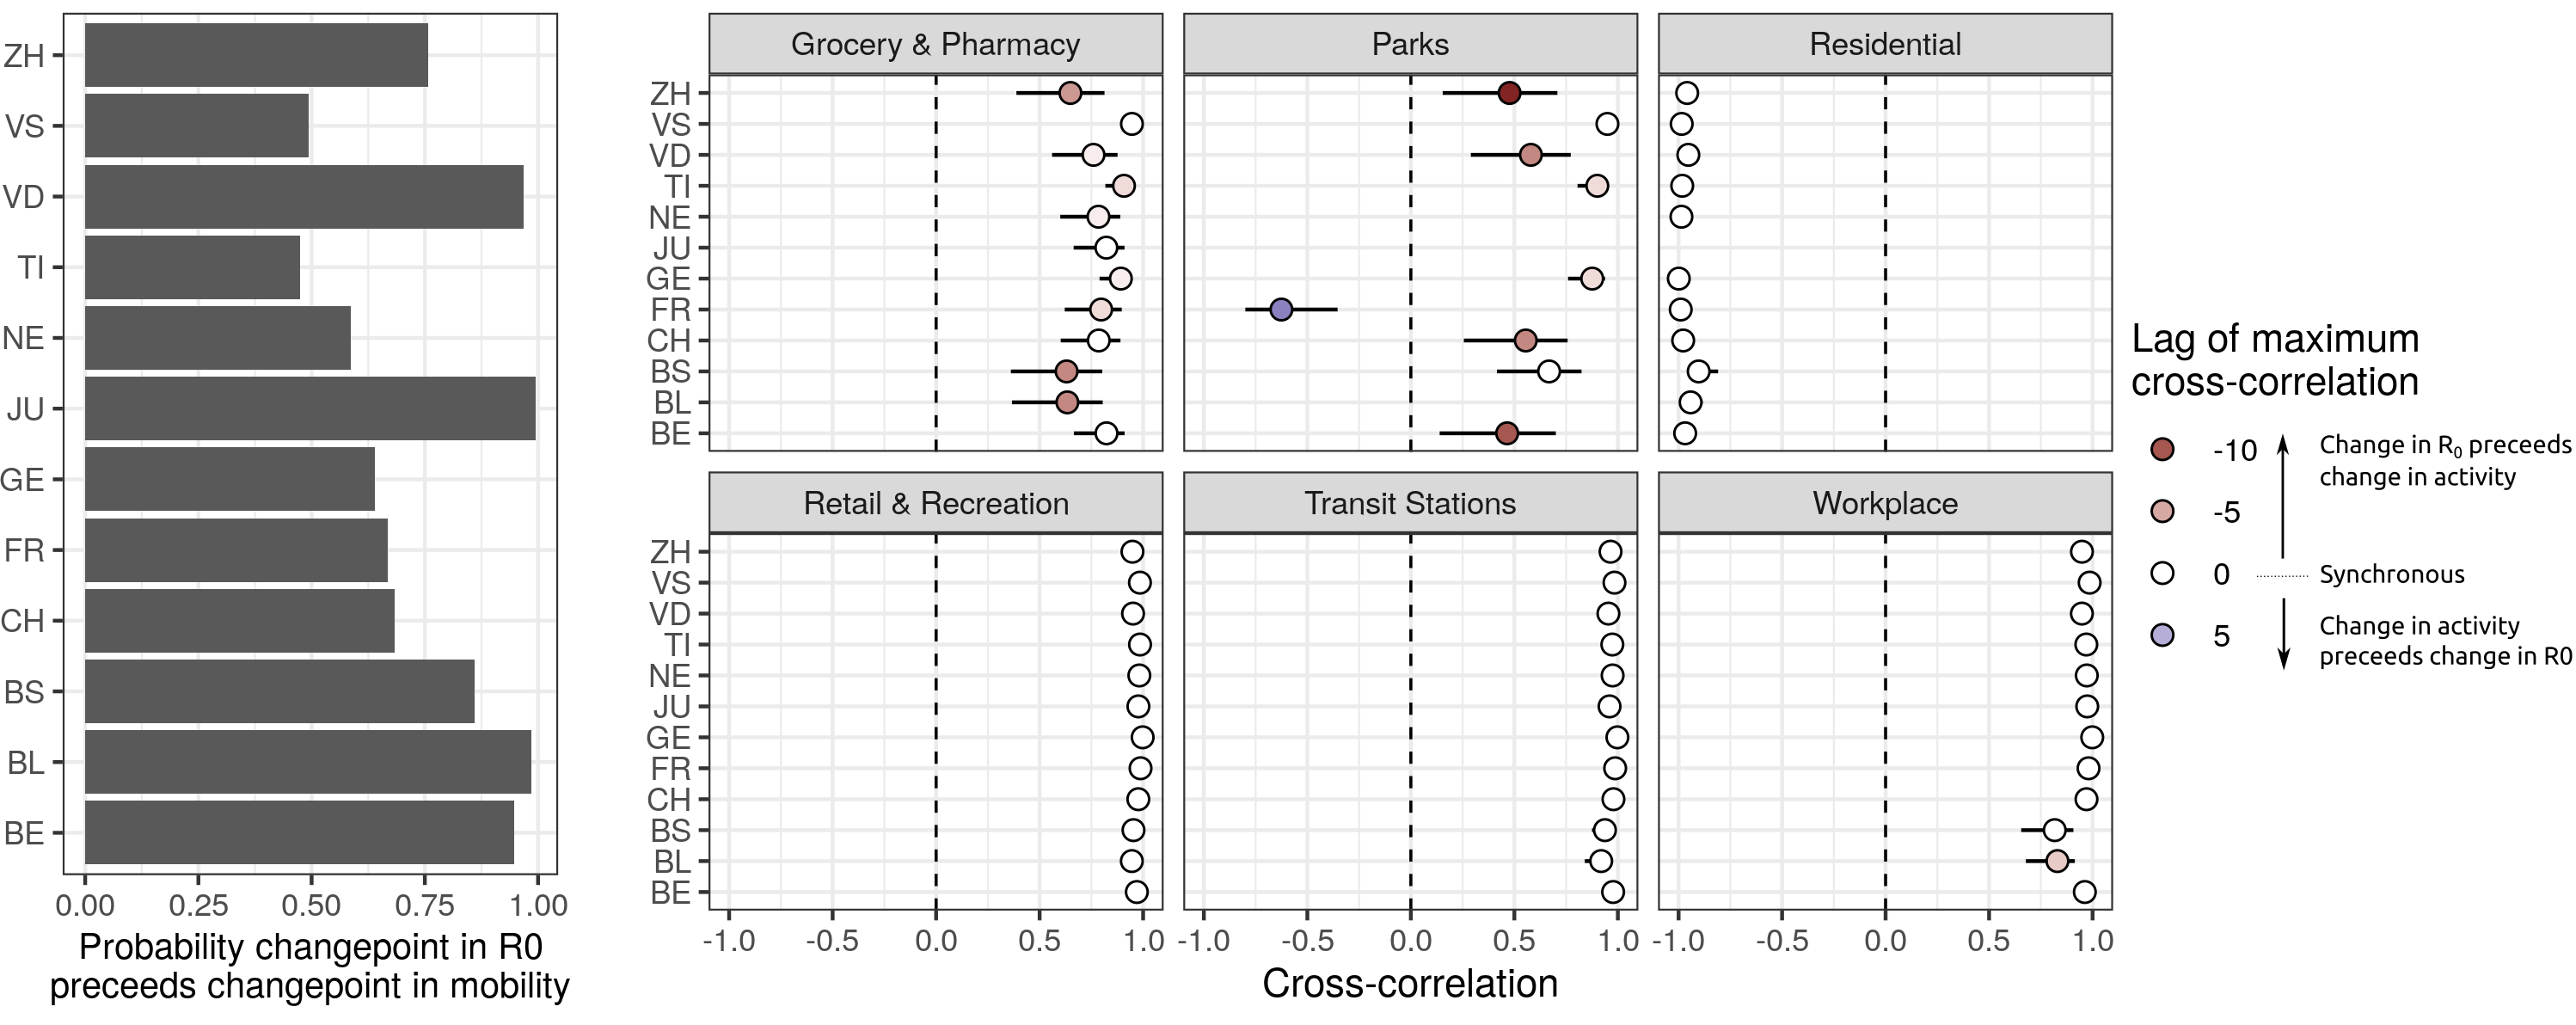
\includegraphics[width=\textwidth]{fig_covid-switzerland-npi/FIGURE_4.png}
  \caption[Timing between changes in R0 and mobility.]{Timing between changes in R0 and mobility. Left: probability that the first changepoint in R0 occured before the first changepoint in mobility-related activity. Right: Maximum cross-correlations between time series of changes in R0 and changes in mobility (bars 95\% CI). Lags refer to the delay between changes in mobility-related activity and changes in R0 (positive lag k indicates that current changes in mobility have maximal cross-correlation with changes in R0 k days in the past).}
  \label{fig:covid-ch-timing}
\end{figure*}

In the majority of cases, correlation between mobility and $R_0$ was strongest with no lag between the two. However, changes in mobility to workplaces lagged behind changes in $R_0$ in Basel-Stadt and Basel-Landschaft. Correlations between changes in $R_0$ and grocery and pharmacy mobility were less marked (national level 0.65), with changes in mobility occurring after changes in $R_0$ (negative lags in fig. \ref{fig:covid-ch-timing}). In most cantons, a strong increase in park mobility after 25 March resulted in a positive correlation with changes in $R_0$, but with negative lags (change in activity after change in $R_0$, fig. \ref{fig:covid-ch-timing}). We did not find significant linear associations between the level of reduction in mobility and maximum reduction in $R_0$ across cantons, except for a small effect size for reduced park mobility (regression coefficient of 0.15, 95\% CI 0.02–0.25) (postprint supplementary fig. 8). We estimated a commonly reported metric, the effective reproduction number (Reff), which is an aggregate measure of transmission capturing aspects of both infectious contacts and of population susceptibility. Across cantons, Reff was extremely close to $R_0$, indicating that a small fraction of the population is expected to have natural immunity to SARS-CoV-2 (as we assumed was true in the short term after infection). We estimated that as of 24 April, 3.9\% (95\% QR 3.6–4.3\%) of the population nationally had been infected, with median estimates ranging from 1.9\% (Bern) to 16\% (Ticino) (fig. \ref{fig:covid-ch-map}). Modelled estimates of the proportion infected of people infected in the canton of Geneva are in agreement with preliminary results from ongoing serological studies, which have estimated the seroprevalence to be 9.7\% (95\% CrI 6.1–13.1\%) in the third week of April\cite[3\baselineskip]{Stringhini:RepeatedSeroprevalenceAntiSARSCoV2:2020}, compared with modeled estimates of 8.9\% (95\% QR 7.8–10.1\%) after accounting for the time from infection to seroconversion\cite{Wolfel:VirologicalAssessmentHospitalized:2020}(postprint supplementary fig. 7).

\begin{figure}\centering
  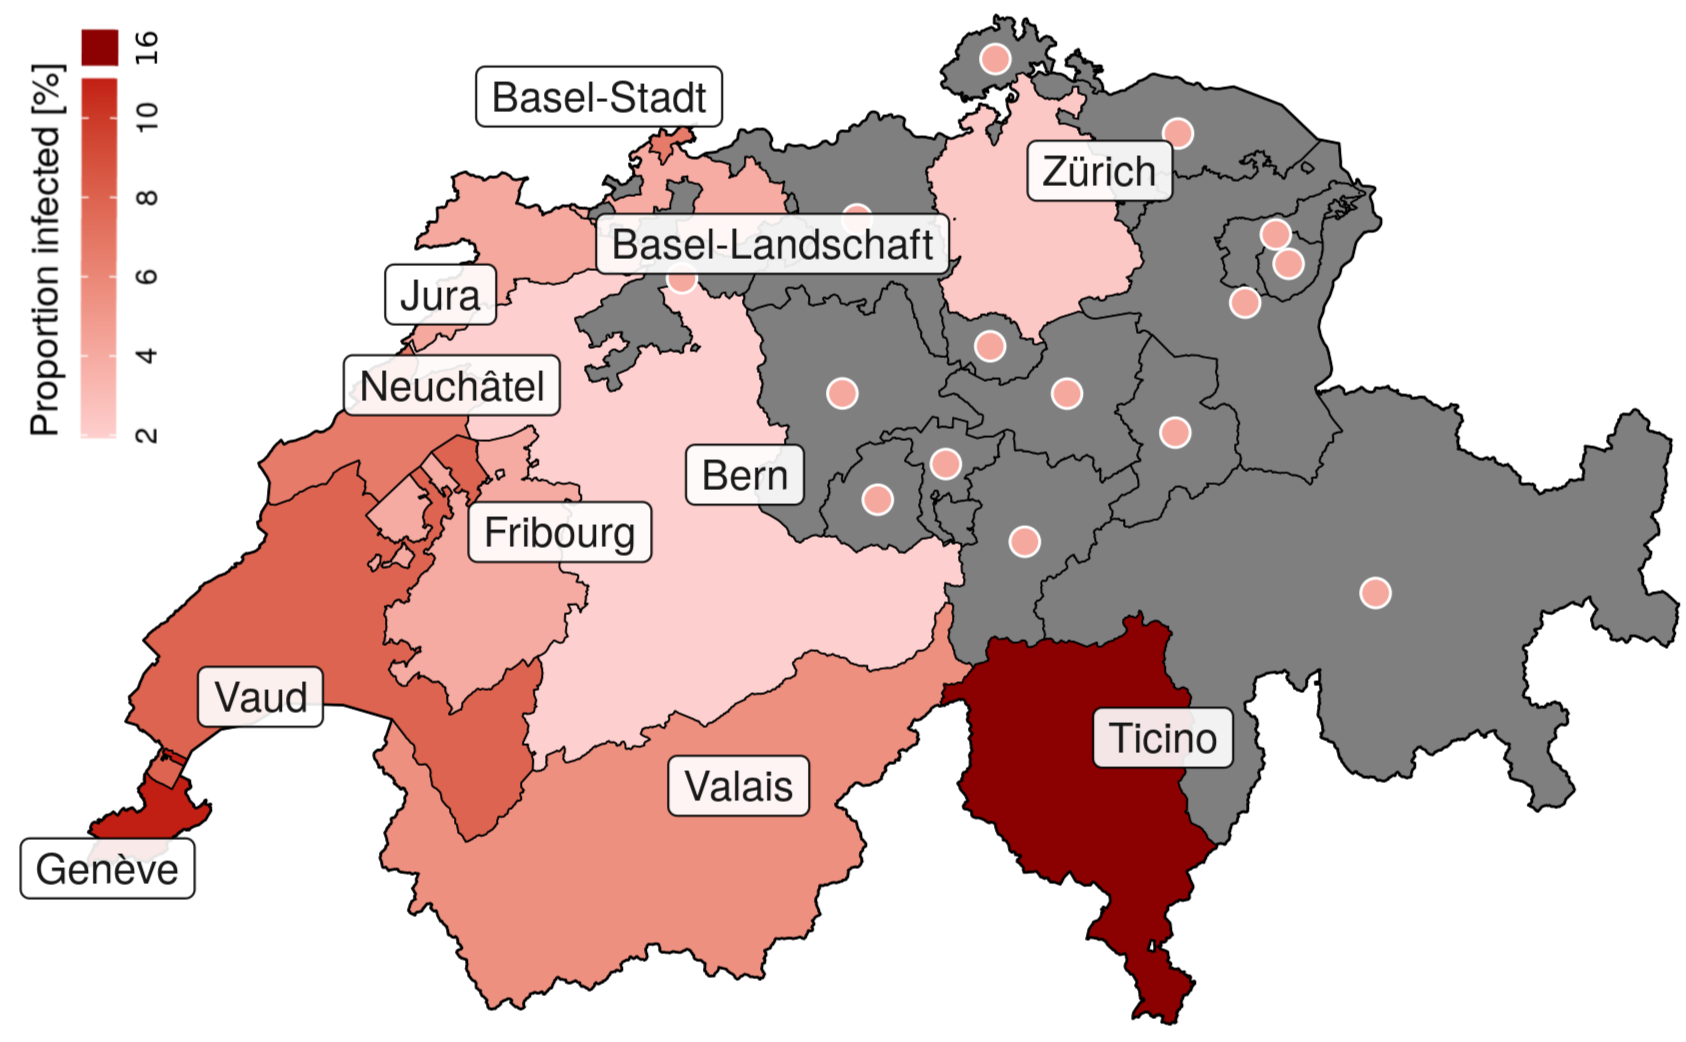
\includegraphics[width=\textwidth]{fig_covid-switzerland-npi/FIGURE_5_mod.png}
  \caption[Modelled proportion of people infected with SARS-CoV-2 in Switzerland.][3\baselineskip]{Modelled proportion of people infected with SARS-CoV-2 in Switzerland up to 24 April. Estimates were produced for 11 of 26 cantons for which enough data were available (unmodelled cantons are shown in gray with points indicating the national-level estimated incidence proportion of 3\%). Values are reported in supplementarytable 6 of appendix 1.}
  \label{fig:covid-ch-map}
\end{figure}

\section{Discussion}
Our results suggest a strong reduction of $R_0$ across Switzerland since the start of the epidemic. The reduction in $R_0$ started around 7 March, thus about 1 week before the implementation of lockdown-type NPIs. Analysis of activity-related mobility data also showed strong support for changes in mobility starting prior to the implementation of most NPIs. Estimated reductions of viral transmission were strongly correlated and mostly synchronous with observed changes in mobility patterns, although the initiation of changes in transmission preceded measurable changes in activity-related mobility. The methods used to infer the time series of $R_0$ do not rely on assumptions on the shape of how it changed in time, nor on the dates at which change started. Alternative methods that rely on fixed dates (such as that of the Imperial College COVID-19 Response Team\cite{Flaxman:Report13Estimating:2020}) might be biased as changes in transmission are not synchronous with policy changes. Distribution based methods such as provided by R package EpiEstim\cite{Wallinga:DifferentEpidemicCurves:2004,Cori:NewFrameworkSoftware:2013} are flexible but subject to bias when misused\cite{Lipsitch:CommentPanLiu:2020}. In addition, our approach enables the estimation of $R_0$, which is a direct quantification of transmission potential, as opposed to the effective reproduction number Reff, which also accounts for the effect of susceptible depletion as done in the above-mentioned statistical approaches. This enabled us to estimate the proportion of reduction in transmission attribuable to behavioural changes, which is therefore more suited to study the impact of NPIs. Aside from these methodological differences, our estimates are in line with other estimates in Switzerland: Althaus et al.\cite{Althaus:RealtimeModelingProjections:2020} estimated a reduction of 89 \% (83–94\%) from a baseline of 2.78 (2.51–3.11), Scire et al.\cite{Scire:ReproductiveNumberCOVID19:2020} estimated a reduction of 76 \% (70–82\%) from a baseline of 1.88 (1.80–1.98) and Imperial College estimated a reduction of 60\% (50–80\%) from a baseline of 3.5 (2.8–4.3)\cite{Flaxman:Report13Estimating:2020}. Our results provide strong support for a reduction of transmission starting about 1 week prior to school closure, the first national-level NPI targeting daily activities, which was ordered on 13 March. Moreover, initiation of transmission reduction was found to precede changes in mobility patterns as detectable from the Google dataset. A possible explanation for this initial decrease in transmission could be linked to the strong increase in public interest in COVID-19 in February as measured by Google searches for COVID-19-related keywords.

\begin{marginfigure}[1\baselineskip]
%\centering
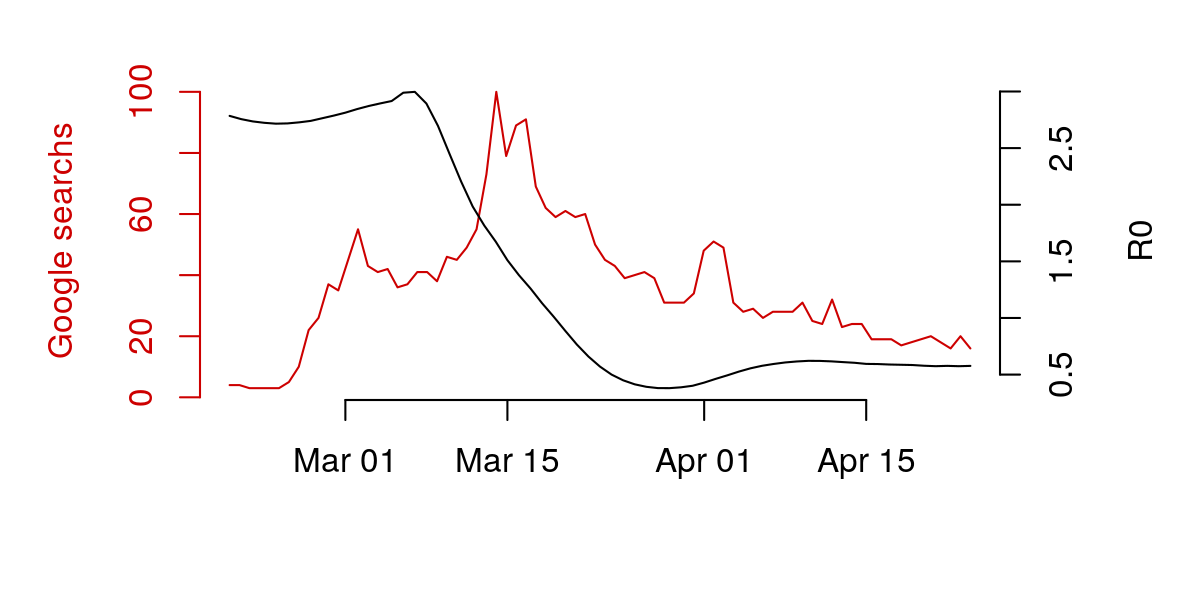
\includegraphics{fig_covid-switzerland-npi/fig_supp/google_trends.png}
\margincaption[Google trends for COVID-19 and changes in R$_0$ in Switzerland]{\footnotesize Google trends for COVID-19 and changes in R$_0$ in Switzerland. Trends corresponds to amount of searches for the keyword "coronavirus" (red line) between February 15 and April 30 and are given as a percent of the maximum number of searches in the period, time evolution of R$_0$.}
\end{marginfigure}
 In fact, we estimated that a second sharp rise in Google searches started on 7 March (95\% CrI 3–9 March), which overlaps with our estimated start of national level decrease in $R_0$ on 7 March (probability that changepoints coincide 0.76). The Federal Office for Public Health issued an information campaign on COVID-19 on 28 February, which was updated on 2 March to stress basic hygiene rules\cite{OFSP:NouvellesReglesHygiene:2020}. This may have resulted in voluntary social distancing as well as increased hygiene early on without noticeable changes in mobility patterns. This type of proactive change in behaviour would be in line with early changes in mobility patterns, which were estimated to precede school closures and subsequent measures. Our results suggest that the value of $R_0$ was likely already below one on 20 March, when the federal government banned gatherings of more than five people and recommended voluntary home isolation for the whole population. This result should however be taken within context, as the announcement was anticipated on social networks earlier that week, and so was probably already impacting social distancing behaviour. We therefore recommend caution in any causal interpretation of our results on the role of this last NPI on driving $R_0$ below one. Despite the strong association between the changes in mobility and reductions in $R_0$ within each canton, the lack of cross-cantonal associations between the level of reduction in mobility types and the level of reduction in $R_0$ suggests context-specific pathways between COVID-19 transmission and mobility intensity. This warrants caution in attempting to apply general relations between mobility and transmission reduction. Investigation of general associations will require more in-depth studies controlling for other factors such as population density, economic activities and social mixing patterns, and inter-cantonal mobility patterns, in addition to incorporation of potential environmental drivers of transmission such as temperature and relative humidity\cite{Neher:PotentialImpactSeasonal:2020, Kissler:ProjectingTransmissionDynamics:2020}. We note several limitations to this work. First, due to the relatively recent introduction of SARS-CoV-2 in Switzerland compared with the length of hospital and ICU stays, the time distribution of hospital in- and out-patients is biased towards shorter duration (postprint supplementary fig. \ref{fig:covid-ch-mobility}), which we addressed by accounting with right-censoring using survival models. In addition, because of the limited data available in some places, we were only able to fit our model for 11 of the 26 cantons. Modelling results presented in this work are subject to our hypothesis on yet uncertain parameters of COVID-19, including the infection fatality rate and the proportion of severe infections requiring hospitalisation. An important uncertainty is the fraction of asymptomatic infections and their relative contribution to disease transmission. We currently assume that all infected individuals contribute equally to transmission, which means our estimate of the proportion of people infected would under-estimate true cumulative incidence if there were a large fraction of asymptomatic infections with a relatively low contribution to transmission. Evidence from South Korea, however, suggests that only a small fraction (2\%) of confirmed COVID-19 infections are totally asymptomatic, and none of the household members of these asymptomatic carriers were infected\cite{Park:EarlyReleaseCoronavirus:2020}. Moreover, model results are in agreement with preliminary results from ongoing serological studies in Switzerland\cite{Stringhini:RepeatedSeroprevalenceAntiSARSCoV2:2020}. Moreover, our estimates of time-varying basic reproduction numbers assume that the generation interval for COVID-19 in Switzerland remained unchanged, thus potentially ignoring the joint role of $R_0$, the infectious period and contact rates in determining the disease’s intrinsic growth rate\cite{Yan:SeparateRolesLatent:2008}. If it is assumed that the generation interval increased with the reduction of social contact, our estimates are conservative overestimates of the “true” value of $R_0$, which is encouraging from a public health perspective. Inferred disease dynamics and estimated time-varying $R_0$ also depend on the values of the incubation period, which we set to the estimates currently available in the literature. In our modelling framework, we estimated the initial conditions along with changes in $R_0$, which could, however, be influenced by the role of imported cases in driving disease dynamics, especially in cantons bordering regions with strong COVID-19 transmission in early February (Eastern France for Basel-Stadt and Basel-Landschaft and Northern Italy for Ticino). Since we did not model importations, this could yield an overestimation of the initial value of $R_0$, which warrants caution in interpreting specific values of $R_0$ in these cantons. This potential overestimation would, however, not affect the strong inferred reduction in $R_0$. Another limitation of our study is that it was not possible to disentangle the individual contribution of each NPI on $R_0$ in this analysis owing to the early onset of changes in $R_0$ and in mobility patterns, as well as the very close spacing between the different types of NPI. This information would, however, be extremely valuable in supporting decisions on NPI strategies against COVID-19. Efforts to constitute a global database of NPIs will provide the opportunity to extend this type of analysis to other settings and produce evidence for the effect of different types of NPIs\cite{HITCOVIDTeam:HealthInterventionsTracking:2020}. As the Swiss government plans to gradually lift restrictions, close monitoring of changes in $R_0$ is critical, given that the reductions in transmission appear to be almost entirely driven by changes in behaviour, not through herd immunity. Near real-time estimates of $R_0$ may serve as a critical tool for public health and political decision makers in the months to come, and efforts should be made to refine models like ours using new data, including those from population-based serological studies, mobility data and more detailed individual-level data on COVID-19 cases across the spectrum of severity.\marginnote{While relying on hospitalization and death allowed for an early robust identification of the basic reproduction number, it would be necessary to add a reporting process and case data to update our estimate through 2020-2021. Convolution-based methods are more convenient to maintain, and very good continuous updates of the reproduction number in Switzerland available on the Swiss National COVID-19 Task Force website \url{sciencetaskforce.ch/en/current-situation/}. It is provided by the ETHZ, with method described in\fullcite{Huisman:EstimationWorldwideMonitoring:2021}.}

